%!TEX program = xelatex
\documentclass[10pt, compress]{beamer}
\usetheme[titleprogressbar]{m}
%\usetheme{CambridgeUS}

\usepackage{booktabs}
\usepackage[scale=2]{ccicons}
\usepackage{minted}
\usepackage[utf8]{inputenc}
\usepackage{lmodern}
\usepackage[spanish, mexico]{babel}
%\usepackage{color}
%\usepackage[usenames,dvipsnames,svgnames,table]{xcolor}

\usepackage{enumitem}
\setlist[itemize,1]{label={\fontfamily{cmr}\fontencoding{T1}\selectfont\textbullet}}
\setlist[itemize,2]{label=\textopenbullet}
\setlist[itemize,3]{label=\textopenbullet}

\setbeamercolor{block title}{use=structure, bg=orange!50,fg=black}
%\setbeamercolor{block title}{use=structure, bg=gray!40,fg=black}
\setbeamercolor{block body}{use=structure, bg=gray!20,fg=black}
%\setbeamercolor{structure}{fg=darkred}

\usepgfplotslibrary{dateplot}

\usemintedstyle{trac}

\title{\sc DETECCIÓN DEL ROSTRO HUMANO, ESTIMACIÓN DE SU POSE Y DE SU MIRADA}
\subtitle{Avances de Tesis}
\author{Rajiv González}
\institute{Maestría en Ciencias de la Computación, UADY}

\begin{document}

\maketitle

\begin{frame}[fragile]
	\frametitle{Introducción}
	\begin{itemize}
		\item ¿Por qué una persona mueve su cabeza?
		\item Importancia de conocer la posición y orientación
		\item Mediante imágenes capturas de personas es posible conocer la posición y orientación de su cabeza.

		\begin{figure}[htbp]
			\centering
			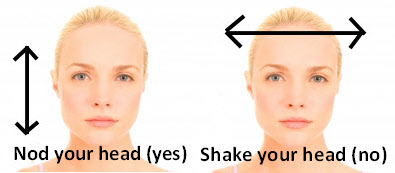
\includegraphics[width=.5\textwidth]{./pictures/nod}
		\end{figure}
	\end{itemize}

\end{frame}

\begin{frame}[fragile]
\frametitle{Objetivo}

  \begin{block}{hola}
  Detectar el rostro de las personas y estimar su pose mediante una cámara monocular con el objetivo de inferir la región que estén mirando en un plano virtual enfrente de ellas.
  \end{block}



%\begin{figure}
%  \centering
%% \includegraphics[width=6cm,height=6cm]{firstex.png}
%\end{figure}

\end{frame}
%\section{Metodología}
\begin{frame}[fragile]
\frametitle{Titulo}
%\setbeamerfont{framesubtitle}{subtitulo}
a

\end{frame}
\plain{Questions?}



\end{document}